

\section{Démarrage}
\subsection{Obtenir le droit d'accès / Demander un nouveau mot de passe}

% Die Zugangsberechtigung zum CUBE PA erhalten Sie für das Projekt Zugkunft Waldenburgerbahn beim Gesamtleiter. Senden Sie
% eine E-Mail an folgende Adresse (Zeitpunkt der Aufschaltung wird noch bekanntgegeben):

Le droit d'accès à CUBE PA vous est donné par le responsable du projet. Si vous avez des questions concernant les responsabilités ou la version d'un accès CUBE PA, vous pouvez vous adresser à l'adresse e-mail suivante :

\vspace{\baselineskip}

% \href{mailto:cube.support@emchberger.ch}{\textstyleInternetlink{cube.support@emchberger.ch}}
{\color{red} cube.support@emchberger.ch}

\vspace{\baselineskip}

Si vous avez oublié votre mot de passe, vous pouvez demander un nouveau sur la page de connexion de CUBE PA en cliquant sur 'Mot de passe oublié'. Un lien pour réinitialiser votre mot de passe vous sera envoyé par e-mail. Si vous avez des questions vous pouvez aussi vous adresser à l'adresse e-mail mentionnée plus haut.

\vspace{\baselineskip}

Pour des raisons de sécurité nous vous recommandons de changer immédiatement les mots de passe reçus par e-mail.

\subsection{Connexion Internet}

Une connexion Internet est indispensable pour l'utilisation de CUBE PA. Travailler hors ligne n'est pas pris en charge, vu que toutes les données sont sauvegardés sur un serveur.

\vspace{\baselineskip}

En cas de problèmes imprévus en utilisant CUBE PA, vérifiez le symbole de l'état de la connexion, en bas à droit de l'écran. S'il est rouge, la connexion Internet est interrompue. Si ceci se produit pendant que vous saisissez des données, essayez de rétablir la connexion et cliquez 'Actualiser' pour sauvegarder les données qui se trouvent encore dans la mémoire locale de CUBE PA. Si vous n'arrivez pas à rapidement rétablir la connexion, ne quittez pas CUBE PA et n'éteignez pas votre ordinateur. Cherchez un autre lieu où vous pouvez établir une connexion et cliquez 'Actualiser' dès que vous l'avez établie.

\vspace{\baselineskip}

\textbf{Etat de la connexion :}

\vspace{\baselineskip}

\begin{tabular}{c | p{14cm} l} %{cl}

\vspace{+1pt}	

\includegraphics[height=12pt] {/Icons/online.jpg} & La connexion Internet est établie et vous êtes connecté à CUBE PA. \\
\vspace{+1pt}	

\includegraphics[height=12pt]{/Icons/offline.jpg} & La connexion Internet est interrompue ou le serveur CUBE PA est momentanément inaccessible. \\
\vspace{+1pt}	

\includegraphics[height=12pt]{/Icons/abgemeldet.jpg} & Le symbole de statut ne s'affiche pas, votre connexion Internet est établie mais vous n'êtes pas connecté à CUBE PA. \\

% 
\includegraphics[height=12pt]{/Icons/BlaueWolke_Blitz.jpg} & Sie haben eine Internet-Verbindung, sind aber nicht in CUBE PA angemeldet \\

\end{tabular}

\vspace{\baselineskip}

Si vous quittez CUBE PA pendant que la connexion Internet est interrompue, les données que vous venez de recenser seront perdues.

\subsection{Démarrer CUBE PA}

% Benutzerspezifisch

Vous pouvez accéder à CUBE PA par l'adresse suivante :

\vspace{\baselineskip}

{\color{red} http://www.cubetools.ch/}

\vspace{\baselineskip}

Vous serez dirigé vers la page d'accueil CUBE Tools :

\begin{figure}[H]
\center{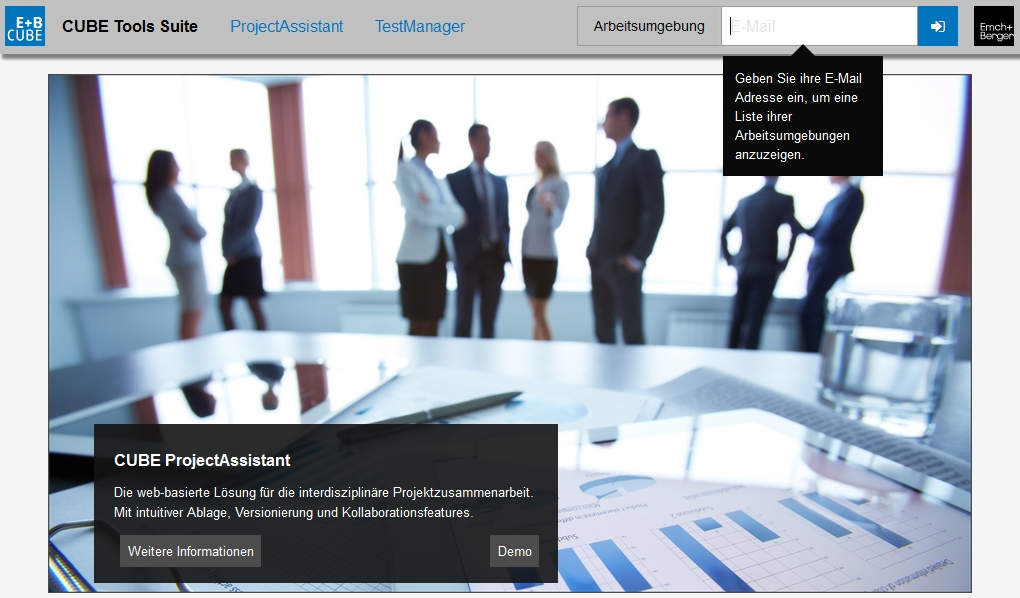
\includegraphics[width=1\linewidth]{../chapters/02_GettingStarted/pictures/2-3_Einstiegsseite.jpg}}
\caption{La page d'accueil CUBE Tools}
% \label{fig:speciation}
\end{figure}

Saisissez votre adresse e-mail en haut à droite et cliquez sur la flèche bleue :

\begin{figure}[H]
\center{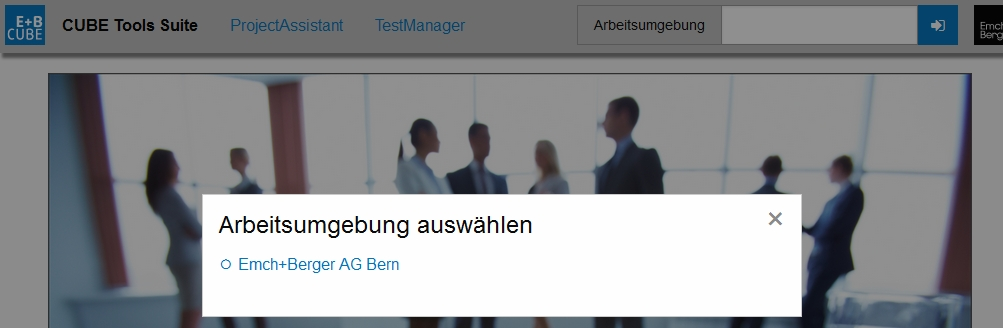
\includegraphics[width=1\linewidth]{../chapters/02_GettingStarted/pictures/2-3_Arbeitsumgebung_auswaehlen.jpg}}
\caption{Choisir l'environnement de travail}
% \label{fig:speciation}
\end{figure}

Tous les environnements de travail dans lesquels vous êtes enregistré sont affichés. Cliquez sur l'environnement de travail souhaité. Vous êtes dirigé vers la page de connexion CUBE PA :

\begin{figure}[H]
\center{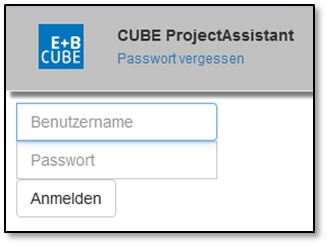
\includegraphics[width=0.35\linewidth]{../chapters/02_GettingStarted/pictures/2-3_CUBEPA_Anmeldung.jpg}}
\caption{Se connecter à CUBE PA}
% \label{fig:speciation}
\end{figure}

Saisissez votre nom d'utilisateur et votre mot de passe. Après avoir cliqué sur 'Connexion', votre aperçu personnel s'affiche.

\subsection{Changer le mot de passe}
\label{bkm:Ref434828103}

Pour des raisons de sécurité nous vous recommandons de changer immédiatement les mots de passe reçus par e-mail. Pour changer votre mot de passe, cliquez sur votre nom en haut de la page. Le menu déroulant qui s'affiche vous permet de vous déconnecter de CUBE PA, de changer votre mot de passe et d'ouvrir ou de sauvegarder le présent manuel.

\begin{figure}[H]
\center{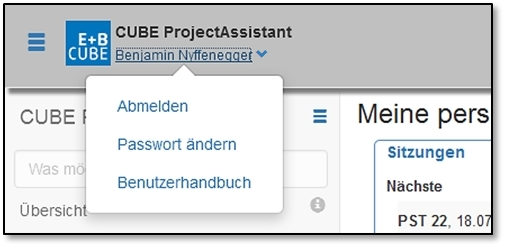
\includegraphics[width=0.5\linewidth]{../chapters/02_GettingStarted/pictures/2-4_Passwort_aendern.jpg}}
\caption{Changer le mot de passe}
% \label{fig:speciation}
\end{figure}

Quand vous cliquez sur 'Changer mot de passe' un masque de saisie apparaît. Vous devez y saisir votre mot de passse actuel une fois et votre nouveau mot de passe deux fois :

\begin{figure}[H]
\center{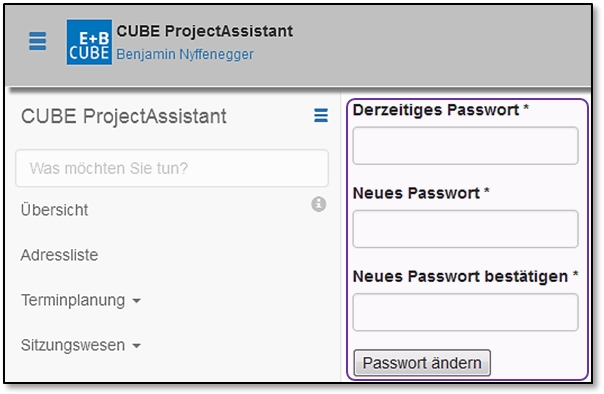
\includegraphics[width=0.5\linewidth]{../chapters/02_GettingStarted/pictures/2-4_Passwort_Eingabe.jpg}}
\caption{Enregistrer le nouveau mot de passe}
% \label{fig:speciation}
\end{figure}

Le nouveau mot de passe devient valable une fois que vous aurez cliqué sur 'Modifier le mot de passe'.

\subsection{Les menus, boutons et symboles les plus importants en bref}

L'utilisation de CUBE PA est orientée vers l'utilisation des applications Internet courantes. Si vous utilisez un smartphone ou une tablette vous devrez facilement naviguer vous repérer sur CUBE PA.

\vspace{\baselineskip}

Dans ce chapitre, les menus, boutons et symboles les plus importants sont décrits lorsqu'ils apparaissent partout dans CUBE PA et qu'ils ont toujours la même signification.

\pagebreak

\subsubsection{Menus}

\begin{figure}[H]
\center{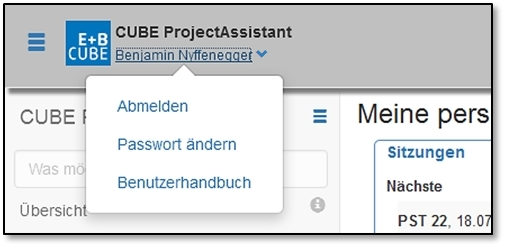
\includegraphics[width=0.5\linewidth]{../chapters/02_GettingStarted/pictures/2-4_Passwort_aendern.jpg}}
\caption{Le menu d'accès}
% \label{fig:speciation}
\end{figure}

Le nom de la personne connectée à CUBE PA apparaît en haut à gauche. Cliquez dessus et un menu déroulant apparaît. Vous pouvez alors changer le mot de passe comme décrit plus haut (Chapitre \ref{bkm:Ref434828103}). Cliquez sur 'Manuel d'utilisateur' pour ouvrir le présent manuel ou le sauvegarder sous format PDF. Si vous cliquez sur 'Déconnexion', vous quittez CUBE PA, sauf si vous n'avez pas encore sauvegardé des données récemment saisies. Dans ce cas un avertissement apparaît :

\begin{figure}[H]
\center{\includegraphics[width=1\linewidth]{../chapters/02_GettingStarted/pictures/251_Browsermeldung.jpg}}
\caption{Avertissement du navigateur}
% \label{fig:speciation}
\end{figure}
\begin{small}
Le contenu de cet avertissement dépend du navigateur utilisé (ici Firefox) et ne peut pas être influencé.
\end{small}

\vspace{\baselineskip}

Vous pouvez interrompre la déconnexion de CUBE PA (rester sur la page) et sauvegarder les données en cliquant sur 'Actualiser'.

\vspace{\baselineskip}

\pagebreak

A gauche se trouve le menu principal :

\vspace{\baselineskip}

\begin{wrapfigure}[20]{l}{6.5cm}   % [x] Wie manche Zeile soll sich um die Grafik "brechen"
  \vspace{-35pt}      % Grundwert war 20; mit 30 schön oben beim Text ausgerichtet
  \begin{center}
    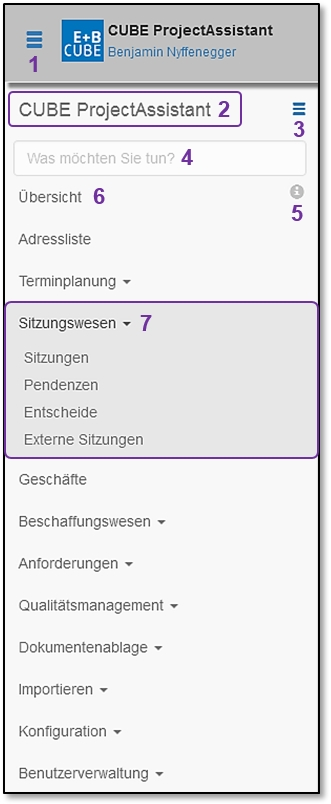
\includegraphics[width=1\linewidth]{../chapters/02_GettingStarted/pictures/2-5-1_Menu_Uebersicht.jpg}
  \end{center}
  \vspace{-20pt}
  \caption{Utiliser le menu}
  \vspace{-10pt}
\end{wrapfigure}

Le menu permet la sélection de tous les domaines auxquels vous avez accès. Par conséquent, l'image présentée ici peut différer de votre menu. Il est également possible que les sous-éléments dans le menu (dans cet exemple 'Séances externes' sous 'Gestion de séances') diffèrent, vu que des éléments de menu additionnels peuvent être configurés spécifiquement pour un client. Les fonctions de base restent cependant toujours les mêmes. Le menu principal peut être affiché et masqué en cliquant sur le symbole de menu \col{(1)}. Ceci est pratique si vous avez besoin d'une plus grande surface de travail dans votre navigateur. \\
La désignation \col{(2)} vous montre votre environnement de travail actuel. En cliquant sur le symbole \col{(3)} vous pouvez directement changer d'environnement de travail.

\vspace{\baselineskip}

\begin{raggedleft}
\hspace{80mm} 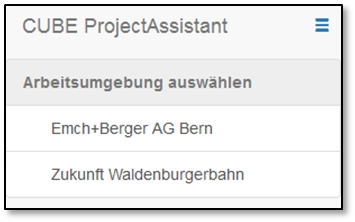
\includegraphics[height=40mm]{../chapters/02_GettingStarted/pictures/2-5-1_Arbeitsumgebung_wechseln.jpg}
\end{raggedleft}

\vspace{\baselineskip}

Vous pouvez uniquement voir les environnements de travail auxquels vous avez accès. Cliquez sur l'environnement de travail souhaité et vous serez dirigé vers la page de connexion correspondante. Si vous avez déjà ouvert un environnement de travail le même jour, sans avoir redémarré votre ordinateur, vous pouvez y accéder sans passer par la page de connexion. Cliquez sur le même symbole \col{(3)} pour fermer la sélection d'environnement de travail. 

\vspace{\baselineskip}

Un outil important est le champ de recherche 'Que voulez-vous faire?' \col{(4)}. Le symbole info \col{(5)} offre des informations utiles pour une recherche productive et effective :

\begin{figure}[H]
\center{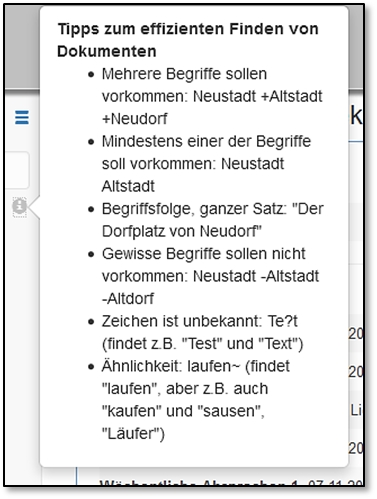
\includegraphics[width=0.35\linewidth]{../chapters/02_GettingStarted/pictures/2-5-1_Hilfe_zu_Suche.jpg}}
\caption{Astuces pour une recherche efficace}
% \label{fig:speciation}
\end{figure}

Cliquez n'importe où dans la fenêtre de navigateur pour fermer la fenêtre info. Saisissez le(s) terme(s) recherché(s) dans le champ de recherche \col{(4)}. CUBE PA parcours tous les éléments de menu et toutes les saisies, ainsi que le contenu des documents téléchargés (par exemple documents Word et PDF). \\

\textbf{Il faut souligner que} les documents PDF ne peuvent être parcourus que lorsqu'il consistent en un texte intégré et non en images. Si un texte a été scanné et sauvegardé comme image dans un ficher PDF, ce document ne sera pas parcouru. \\

\begin{wrapfigure}[14]{r}{7cm}   % [x] Wie manche Zeile soll sich um die Grafik "brechen"
  \vspace{-30pt}      % Grundwert war 20; mit 30 schön oben beim Text ausgerichtet
  \begin{center}
    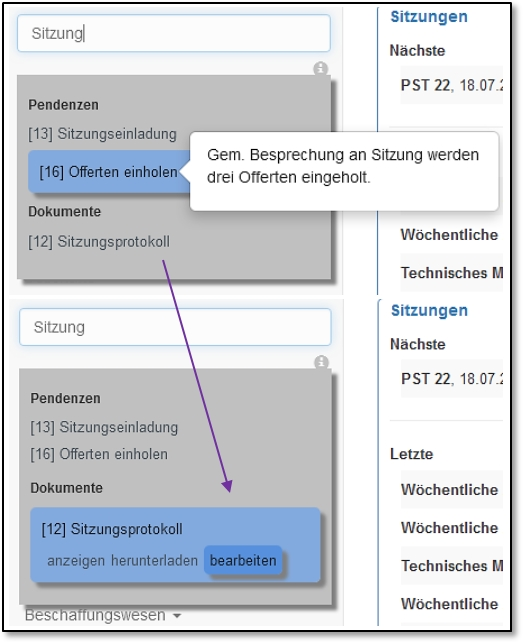
\includegraphics[width=0.8\linewidth]{../chapters/02_GettingStarted/pictures/2-5-1_Such_Ergebnisse.jpg}
  \end{center}
  \vspace{-20pt}
  \caption{Utiliser les résultats de la recherche}
  \vspace{-10pt}
\end{wrapfigure}

Toutes les résultats corresondant aux termes de recherche seront affichés :

\begin{compactitem}
	\item Avec ce mot-clé des résultats ont été trouvés dans les affaires en suspens et dans les documents.
	\item Si vous passez le curseur au dessus de la saisie dans les affaires en suspens, ses détails de apparaissent.
	\item Dans les autres domaines, dans ce cas sous 'Documents', vous avez la possibilité d'afficher, de télécharger ou de modifier le document trouvé. Cliquez ensuite sur l'option souhaitée.
\end{compactitem}

\vspace{\baselineskip}

L'élément de menu 'Aperçu' \col{(6)} vous permet toujours de retourner à votre aperçu personnel. Si un élément de menu comporte des sous-éléments, ceci est indiqué par un petit triangle. Cliquez sur l'élément pour faire apparaître ses sous-éléments \col{(7)}. L'élément 'Gestion de séances' n'est pas un lien en soi. Cliquez à nouveau sur l'élément pour masquer ses sous-éléments.

\vspace{\baselineskip}

Le menu principal vous donne accès aux différentes parties de CUBE PA. Selon des droits d'accès qui vous ont été attribués, tous les domaines ne vous seront pas visibles et accessibles.

\begin{itemize}
\item
\textbf{Aperçu}: Affichage des séances, documents et affaires en suspens qui vous concernent.
\item
\textbf{Liste d'adresses}: Affichage des adresses avec fonction de filtre. De nouvelles saisies (personnes et unités d'organisation) peuvent être créées ici.
\item
\textbf{Planning}: Affichage et modification de calendriers.
\item
\textbf{Gestion de séances}: Affichage et modification d'invitations de séances, de procès-verbaux, des affaires en suspens et des décisions.
\item
\textbf{Fonction d'acquisition}: Traitement d'acquisitions, de la publication à l'adjudication.
\item
\textbf{Exigences}: Accès aux documents relatifs aux exigences.
\item
\textbf{Gestion de la qualité}: Accès aux documents relatifs à la gestion de risques et aux interfaces. Le manuel du projet et autres manuels peuvent être chargés ici.
\item
\textbf{Classement des documents}: Gestion de documents avec une vue en ligne. Des documents modifiés sont classés avec un nouveau numéro de version.
\item
\textbf{Importer}: Importation de données (planning et transactions).
\item
\textbf{Configuration}: Définition et gestion du contenu des listes de sélection.
\item
\textbf{Gestion des utilisateurs}: Gestion des utilisateurs, équipes et groupes.
\end{itemize}

% bishierher

\subsubsection{Boutons}

Les boutons suivants sont toujours utilisés :

\vspace{\baselineskip}

% 2.8, 12

\begin{tabular}{|c | p{10cm}|l} %{cl}
\hline
\raisebox{-1\totalheight}{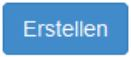
\includegraphics[height=20pt]{/Icons/B_Erstellen.jpg}} & Créer : En cliquant ce bouton, vous sauvegardez une nouvelle saisie pour la première fois, avec l'option de la modifier plus tard. \\
\hline
\raisebox{-1\totalheight}{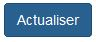
\includegraphics[height=20pt]{/Icons/B_Uebernehmen.jpg}} & Actualiser : En cliquant ce bouton, les saisies que vous avez effectuées récemment et qui se trouvent dans la mémoire locale de votre ordinateur sont sauvegardées sur le serveur. \\
\hline
\raisebox{-1\totalheight}{
\includegraphics[height=20pt]{/Icons/Lupe_s.jpg}} & Loupe : En cliquant la loupe, vous filtrez une liste d'après les mot-clés ou les critères de filtrage saisis dans les champs de la première ligne. \\
\hline
\raisebox{-1\totalheight}{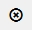
\includegraphics[height=20pt]{/Icons/FilterLoeschen.jpg}} & Effacer le filtre : En cliquant ce symbole, toutes les saisies dans les champs de recherche sont effacées. \\
\hline
\raisebox{-1\totalheight}{
\includegraphics[height=20pt]{/Icons/Blattsymbol_s.jpg}} & Page cornée : En cliquant ce symbole, une liste correspondant aux critères de filtrage actuels est créée sous format PDF. S'il n'y a pas de filtre activé, la liste entière est générée. \\
\hline
\raisebox{-1\totalheight}{
\includegraphics[height=16pt]{/Icons/weitereSeiten.jpg}} & Pagination : Avec ces boutons vous pouvez avancer ou reculer dans la liste en cliquant 'Prochain' ou 'Précédent', ou choisir une page spécifique en cliquant son numéro de page. Si la liste contient plus que cinq pages, toutes les pages ne sont pas affichées. Dans ce cas, cliquez 'Prochain' ou 'Précédent' jusqu'à ce que la page désirée puisse être choisie.  \\
\hline
\end{tabular}

\begin{figure}[H]
\center{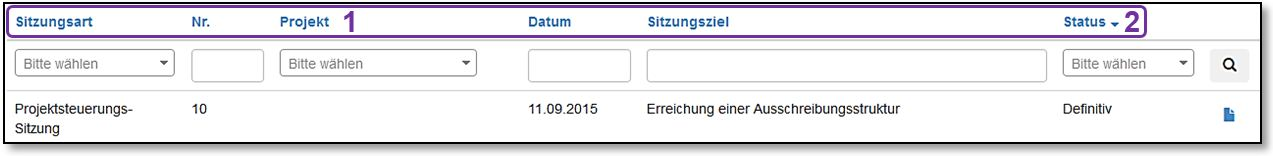
\includegraphics[width=1\linewidth]{252_Listen_sortieren.jpg}}
\caption{Colonnes : Trier le contenu}
% \label{fig:speciation}
\end{figure}


En plus, tous les en-têtes des colonnes en bleu fonctionnent comme un bouton \col{(1)}. En cliquant sur un en-tête de colonne, vous effectuez un tri des éléments de la liste en ordre alphabétique selon les données de cette colonne. Cliquez à nouveau sur l'en-tête pour inverser l'ordre. Le petit triangle 
\includegraphics[height=10pt]{/Icons/welcheSpalte_sort.jpg} \col{(2)} indique selon quelle colonne la liste est triée (la colonne 'Etat' dans cet exemple) et aussi l'ordre du tri : (Ordre A {\textgreater} Z 
\includegraphics[height=10pt]{/Icons/Status_down.jpg} et Z {\textgreater} A 
\includegraphics[height=10pt]{/Icons/Status_up.jpg}).

\pagebreak
\subsubsection{Symboles}
\label{bkm:Ref443039356}
Les symboles suivants ont toujours la même signification. A l'exception des symboles d'état de la connexion Internet, ces boutons et liens changent de couleur quand le curseur de la souris est placé dessus.

\begin{tabular}{|c|p{14cm}|} %{cl}
\hline
\raisebox{-0.5\totalheight}{
\includegraphics[height=12pt]{/Icons/online.jpg}} & Ces flèches vertes se trouvent en bas à droite de la page. Elles signifient que votre connexion Internet est établie et que vous êtes connecté à CUBE PA. \\

\includegraphics[height=12pt]{/Icons/offline.jpg} & Si ces flèches sont rouges, la connexion Internet est interrompue ou le serveur CUBE PA est momentanément inaccessible. \\

\includegraphics[height=12pt]{/Icons/abgemeldet.jpg} & Si vous ne voyez pas les flèches, votre connexion Internet est établie mais vous n'êtes pas connecté à CUBE PA. \\
\hline
\raisebox{-1\totalheight}{
\includegraphics[height=12pt]{/Icons/Plussymbol.jpg}} & Le symbole plus (nouveau) se trouve en haut à gauche d'une fenêtre. Il vous permet de créer une nouvelle saisie (par exemple créer une nouvelle invitation à une séance). \\
\hline
\raisebox{-1\totalheight}{
\includegraphics[height=12pt]{/Icons/Listensymbol_zurueck.jpg}} & Le symbole de liste vous permet de retourner à l'aperçu. Ce symbole est surtout affiché si vous avez ouvert une saisie avec le symbole de la loupe (afficher) ou celui du crayon (modifier). \\
\hline
\raisebox{-1\totalheight}{
\includegraphics[height=12pt]{/Icons/SpaltenEinst.jpg}} & Le symbole de configuration vous permet d'afficher ou de masquer des colonnes d'une liste. Les colonnes qui ne sont pas nécessaires peuvent ainsi être désélectionnées. \\
\hline
\raisebox{-1\totalheight}{
\includegraphics[height=12pt]{/Icons/Stift.jpg}} & Le symbole de crayon se trouve en général dans le coin gauche à côté d'un champ dans une liste. Vous pouvez modifier le contenu de ce champ quand vous cliquez ce symbole. 
\includegraphics[height=14pt]{253_Datum_edit.jpg}\\
\hline
\raisebox{-1\totalheight}{
\includegraphics[height=12pt]{/Icons/Bearbeiten.jpg}} & Crayon encadré (petit) : En cliquant ce symbole (symbole modifier) un masque de saisie s'affiche et vous permet de modifier tous les champs de la donnée choisie. \\
\hline
\raisebox{-1\totalheight}{
\includegraphics[height=12pt]{/Icons/Pluszeichen.jpg}} & Symbole plus : En cliquant sur ce symbole (symbole ajouter) vous pouvez créer une nouvel donnée dans une liste, par exemple un nouveau participant pour une invitation à une séance. \\
\hline
\raisebox{-1\totalheight}{
\includegraphics[height=12pt]{/Icons/Lupe.jpg}} & Symbole loupe : Ce symbole (symbole afficher) se trouve à côté d'une ligne / d'une donnée dans une liste. En cliquant dessus un masque s'affiche et vous permet de lire le contenu de chaque champ de la donnée correspondante. \\
\hline
\raisebox{-1\totalheight}{
\includegraphics[height=12pt]{/Icons/Blattsymbol.jpg}} & Page cornée : Ce symbole apparaît dans un champ dans une liste. Cliquez dessus pour générer un document PDF. Le titre de la colonne indique le contenu du document PDF. \\
\hline
\raisebox{-1\totalheight}{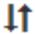
\includegraphics[height=12pt]{/Icons/VertPfeile.jpg}} & Flèches verticales et contraires : Ce symbole vous permet de modifier la position d'une donnée dans une liste. Appuyez ce symbole pour glisser-déposer la donnée à l'endroit voulu. \\
\hline
\raisebox{-1\totalheight}{
\includegraphics[height=12pt]{/Icons/Muelltonne.jpg}} & Poubelle : En cliquant sur ce symbole vous pouvez supprimer une ligne d'une liste et les données qui lui sont associées. Par exemple vous supprimez la saisie d'une pièce-jointe et la pièce-jointe même. Un avertissement de sécurité apparaît : 'Supprimer ?'. Avec la confirmation 'OK', vous supprimez les données. \\
\hline
\raisebox{-1\totalheight}{
\includegraphics[height=12pt]{/Icons/Kreuzchen.jpg}} & Petite croix dans les champs de saisie : En cliquant sur la petite croix dans le coin droit d'un champ vous effacez le contenu d'un champ avec liste de sélection. \\
\hline
\raisebox{-1\totalheight}{
\includegraphics[height=12pt]{/Icons/Pfeil_rechts.jpg}} & Flèche horizontale : Cliquez cette flèche pour afficher un contenu (le rendre visible). \\
\hline
\raisebox{-1\totalheight}{
\includegraphics[height=12pt]{/Icons/Pfeil_unten.jpg}} & Flèche verticale : Cliquez cette flèche pour masquer un contenu (le rendre invisible). \\
\hline
\end{tabular}

\subsubsection{Avertissements et remarques}
Si vous remplissez des champs de saisie dans CUBE PA et vous voulez quitter la page actuelle sans avoir d'abord cliqué 'Actualiser' ou 'Créer', l'avertissement suivant apparaît : 

\begin{figure}[H]
\center{\includegraphics[width=1\linewidth]{251_Browsermeldung.jpg}}
\caption{Avertissement du navigateur}
% \label{fig:speciation}
\end{figure}
\begin{small}
Le contenu de cet avertissement dépend du navigateur utilisé (ici Firefox) et ne peut pas être influencé.
\end{small}

\vspace{\baselineskip}

Vous pouvez alors rester sur la page en cliquant 'Rester sur page' et sauvegarder les données en cliquant sur 'Actualiser' ou 'Créer'. Les données seront autrement perdues.

\vspace{\baselineskip}

Lors de la saisie de données, il y a toujours des champs obligatoires qui doivent être remplis. Si un tel champ obligatoire reste vide, l'avertissement suivant apparaît :

\begin{figure}[H]
\center{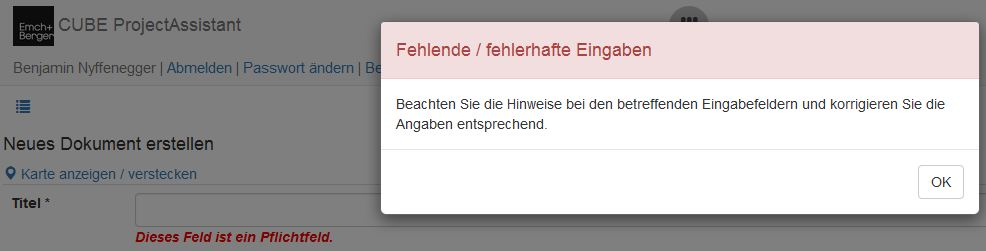
\includegraphics[width=1\linewidth]{254_WarnungPflichfelder}}
\caption{Avertissement de champ obligatoire}
% \label{fig:speciation}
\end{figure}

Le champ à remplir est indiqué en rouge 'Ce champ est un champ obligatoire'. Cliquez 'OK' pour enlever l'avertissement. Vous ne pouvez sauvegarder les données qu'après avoir rempli le champ obligatoire. 


\subsection{CUBE PA sur des appareils mobiles (smartphones, tablettes)}

CUBE PA peut être utilisé sur des appareils mobiles comme des smartphones et des tablettes. CUBE PA reconnaît qu'il s'agit d'un appareil mobile et passe automatiquement à l'affichage 'vue mobile'. Cette vue consiste d'un affichage un peu différent, ainsi que d'un menu adapté (voir ci-dessous). Cependant, si vous utilisez des tablettes sur lesquelles un système d'exploitation Windows ordinaire est installé (par exemple Win 8.1 / Win 10 sur Microsoft Surface), la vue n'est pas changée, ce qui rend CUBE PA difficile à utiliser (CUBE ne peut pas être utilisé ou peut être utilisé uniquement avec saisie tactile).


\begin{figure}[H]
\center{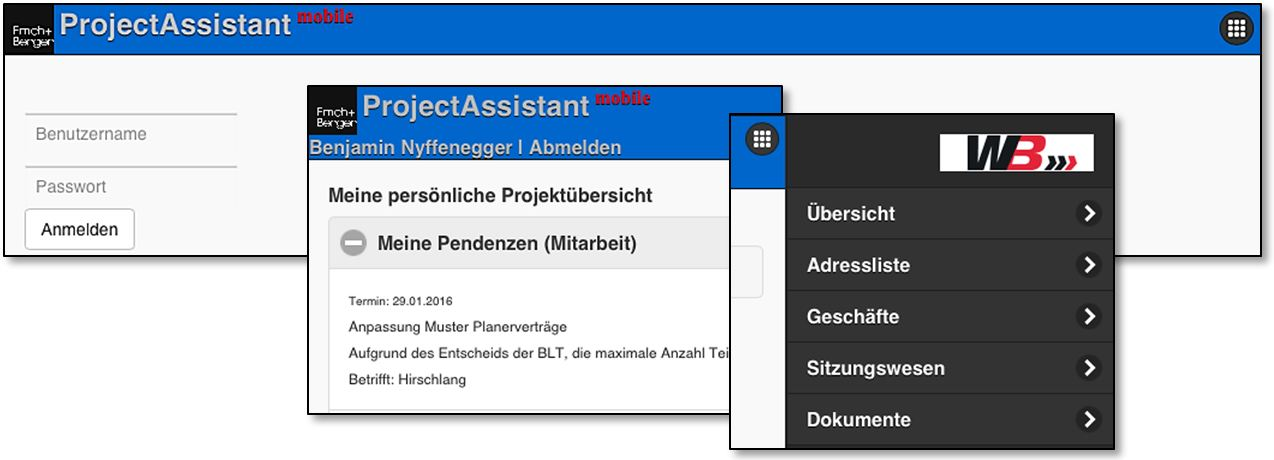
\includegraphics[width=1\linewidth]{26_Mobile_Ansicht.jpg}}
\caption{CUBE PA - la vue mobile }
% \label{fig:speciation}
\end{figure}

\vspace{\baselineskip}

\begin{tabular}{p{7cm} l} %{cl}
CUBE PA sur un iPad: \newline Menu adapté et fenêtre de \newline sélection pour saisie tactile. & \raisebox{-.6\totalheight}{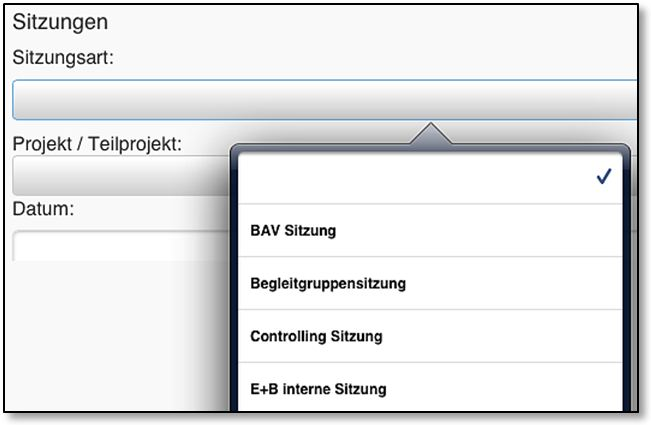
\includegraphics[width=.5\linewidth]{26_iPad_Sitzungen.jpg}}\\
\end{tabular}

\vspace{\baselineskip}

\begin{figure}[H]
\center{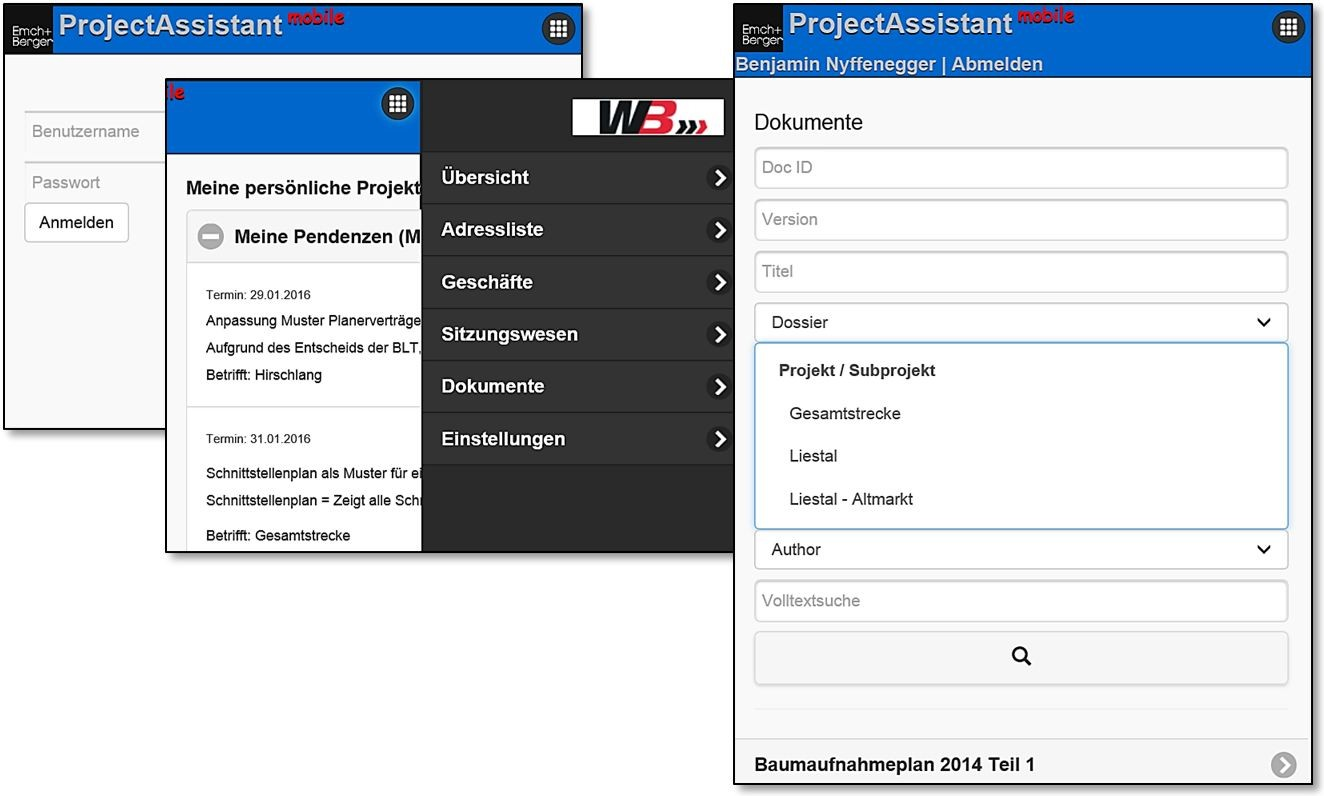
\includegraphics[width=1\linewidth]{26_Mobile_Ansicht2.jpg}}
\caption{CUBE PA - vue mobile sur un smartphone}
% \label{fig:speciation}
\end{figure}

La vue mobile sur un smartphone. Même avec une vue plus petite, CUBE PA s'utilise facilement avec les saisies tactiles et peut afficher les informations nécessaires.
